\section{Versuchsaufbau}
\label{sec:Versuchaufbau}
Für die Messung wird ein Alibava EASy Detekorsystem verwendet. Es
besteht aus einer Detektoreinheit, einer
Kontrolleinheit und einem Computer.
\subsection{Die Detekoreinheit}
Als Detektoreinheit wird ein Halbleitersensor mit
entsprechnender Ausleseelektronik verwendet.
Der Siliziumsensor ist in 128 Streifen unterteilt, jeder ist über
ein Wirebond mit dem Auslesechip (BEETLE) verbunden. Der
BEETLE Chip dient zur Verstärkung des eingehenden Ladungssignals.
Es werden nur Signale an den Computer weitergeleitet, wenn der
Trigger und die Kontrolleinheit in Koinzidenz sind.\\
\subsection{Der Halbleitersensor}
Eine schematische Darstellung des verwendeten Sensors ist in Abbildung
\ref{sensor} dargestellt.
\begin{figure}[H]
  \centering
  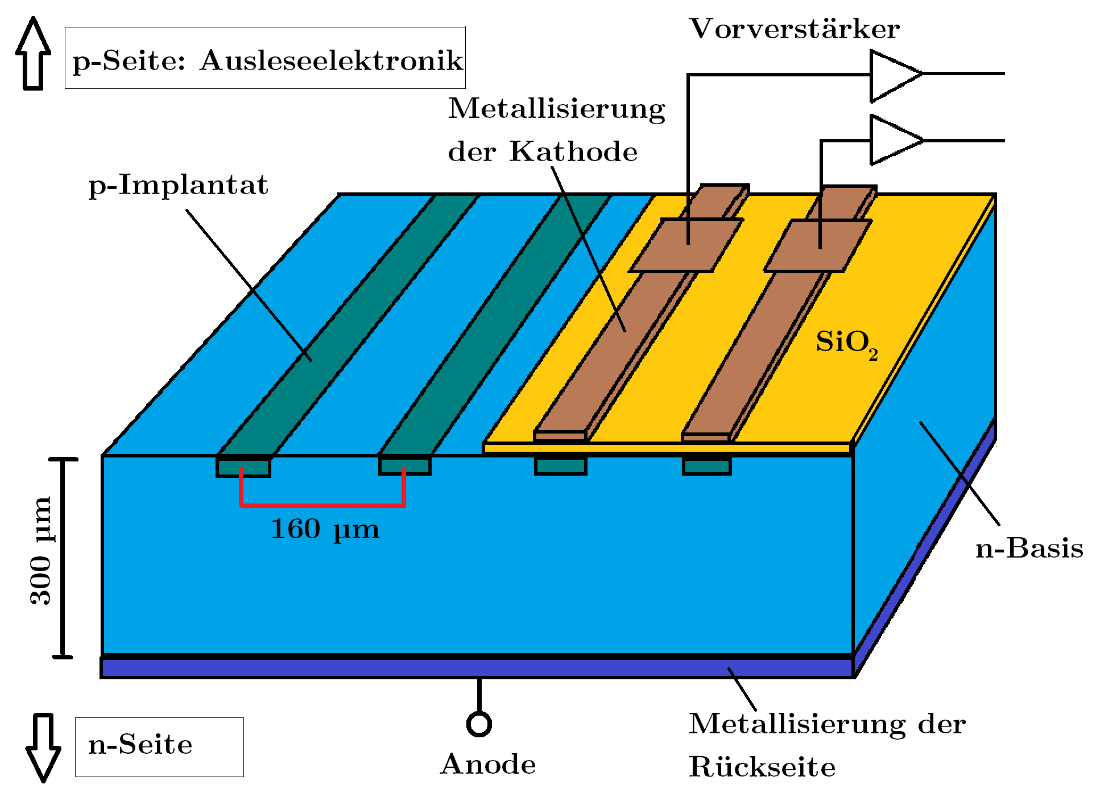
\includegraphics[width=0.81\textwidth]{ressources/sensor.png}
  \caption{Schematische Darstellung des Bändermodells}
  \label{sensor}
\end{figure}
Der pn-Übergang wird hier durch eine n-dotierte Bodenplatte
mit einzelnen p-Implantaten realisiert. Die n-dotierte Siliziumschicht
hat eine Dicke von $300\,\mu m$, die p-Implantate sind von einander isoliert um eine
genaue Ortsauflösung zu ermöglichen. Des Weiteren sind die Implantate
kapazitiv mit einer Elektrode aus Aluminium gekoppelt, was über ein ohmschen Kontakt
ausgelesen werden kann.


Der Sensor muss für die Messung voll depletiert sein, da sonst Elektron-Loch-Paare
außehalb der Depletionszone rekomibinieren. Die Effizienz der Ladungssammlung
$CCE$, steigt mit der Dicke der Depletionszone, bis die Depletionsspannung erreicht ist.
Im Versuch soll die $CCE$ mit Hilfe eines Laser untersucht werden. Hierfür ist die
Eindringtiefe des Laser in Silizium $a$ relevant. Der Zusammenhang ist gegeben durch:

\begin{equation}
    \label{CCE}
    CCE(U)=\frac{1-\exp(\frac{-d_c(U)}{a})}{1-\exp(\frac{-D}{a})}
\end{equation}
Die Eindringtiefe eines Laser der Wellenlänge von 960$\,$nm hat eine Eindringtiefe
von $\approx 74\,\mu$m, wobei dieser Wert vom  Material und der Wellenlänge abhängt.
